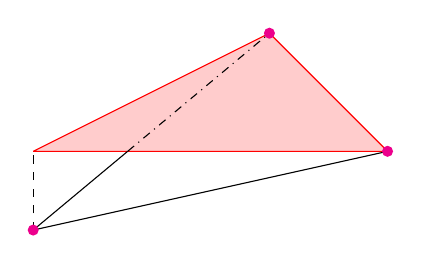
\begin{tikzpicture}	
	\coordinate (A) at (0,0); % pivot
	\coordinate (B) at (3,2.5); 
	\coordinate (C) at (4.5,1);
		
	\coordinate (T) at (0,1);
	
	\draw (A)--(C);
	\draw[dashed] (A)--(T);
	\fill[red!20] (T)--(B)--(C)--(T);
	\draw[red]	(T)--(B)--(C)--(T);
	
	\draw (A)--(1.2,1);
	\draw [dash dot] (1.2,1)--(B);
	
	\foreach \p in {(A),(B),(C)}
		\fill[magenta] \p circle (2pt);
\end{tikzpicture}